\documentclass{rapportCS}
\usepackage{lastpage}
\usepackage{makeidx}
\usepackage{circuitikz}
\usepackage[utf8]{inputenc}
\usepackage{siunitx}
\usetikzlibrary{babel}
\usepackage{titlesec}
\usepackage{array}      % colonnes m{...}
\usepackage[utf8]{inputenc}
\usepackage[T1]{fontenc}
\usepackage{xcolor}
\usepackage{listings}
\usepackage[T1]{fontenc}
\usepackage[utf8]{inputenc} % si tu es en pdfLaTeX
\usepackage{lmodern}
\usepackage{xcolor}
\usepackage{listings}
\usepackage{csvsimple}
\usepackage{amsmath}
\usepackage{siunitx}

% Par exemple : 3 chiffres significatifs
\sisetup{
  round-mode=figures,
  round-precision=4
}

\newcommand{\ResultatsSteelHead}{
  \hline
  Angle~[$^\circ$] & Wmag~[J] & Yba~[Wb] \\
  \hline
}


\lstset{
    language=Matlab,
    basicstyle=\ttfamily\small,
    keywordstyle=\color{blue},
    commentstyle=\color{green!50!black},
    stringstyle=\color{red},
    numbers=left,
    numberstyle=\tiny,
    stepnumber=1,
    numbersep=5pt,
    showstringspaces=false,
    breaklines=true
}
\titleformat{\paragraph}[block]{\normalfont\normalsize\bfseries}{\theparagraph}{1em}{}
\makeindex
\title{Rapport de laboratoire template} %Thanks for Rapport CentraleSupelec - Template, By Axel Poupart-Lafarge
\begin{document}

%----------- Informations du rapport ---------

\logoentreprise{logos/logo_hes.png}

\titre{Rapport de laboratoire} 

\mention{Département TIN}
\trigrammemention{Elmnouar} 
\master{Laboratoire de Systèmes électromécaniques} 
\filiere{3ème année Microtechniques} 

\eleve{Entraînement à moteur pas-à-pas}

\dates{\today}

% Informations tuteurs écoles
\tuteurecole{
    \textsc{Luc Bossoney} \\
   luc.bossoney@heig-vd.ch\\
    \medskip
    \textsc{Gilles Rothermund}\\
    gilles.rothermund@heig-vd.ch\\
   
} 

\tuteurentreprise{
    \textsc{Salma Elmnouar} \\
    salma.elmnouar@heig-vd.ch \\
    \medskip
    \textsc{Julien Golaz}\\
    julien.golaz@heig-vd.ch\\
   
}

%----------- Initialisation -------------------
        
\fairemarges %Afficher les marges
\clearpage 
\fairepagedegarde %Créer la page de garde
\clearpage 
\tabledematieres{}
\listoffigures
\listoftables
\newpage





%------------ Corps du rapport ----------------
\section{Introduction}
\subsection{Contexte}
Dans le cadre du cours \emph{Systèmes électromécaniques}, ce laboratoire porte sur l'analyse et la modélisation d'un entraînement motorisé utilisant un moteur pas-à-pas. 

Ce type de moteur est largement utilisé dans les applications nécessitant un contrôle précis de la position et de la vitesse, telles que la robotique, l'automatisation industrielle, les imprimantes 3D ou les systèmes de manutention. Les moteurs pas-à-pas se distinguent par leur capacité à se déplacer par incréments discrets, appelés pas, ce qui permet un positionnement précis sans nécessité de capteur de retour dans de nombreuses applications. Leur couple varie avec la vitesse, et ils présentent une dynamique particulière, notamment des phénomènes de résonance et de perte de pas, qui doivent être pris en compte lors de la conception de la commande.  

L'étude expérimentale de ce type d'entraînement permet de mettre en pratique les concepts théoriques vus en cours. Elle permet également de comprendre les contraintes propres aux moteurs pas-à-pas et d'appliquer des méthodes de calcul de couple et d'inertie pour dimensionner correctement le système.

\subsection{Objectifs}
Les objectifs de ce laboratoire sont les suivants :
\begin{itemize}
    \item déterminer les différentes inerties mises en jeu dans la chaîne de transmission, y compris celles du moteur, du plateau et des éléments intermédiaires, 
    \item calculer et analyser les profils de couple moteur nécessaires pour atteindre les profils de vitesse spécifiés,
    \item vérifier expérimentalement la limite dynamique pour chaque profil de vitesse, afin de valider les calculs théoriques,
    \item se familiariser avec l'utilisation d'un moteur pas-à-pas piloté par électronique de commande, paramétrable via RS-232, et avec la lecture de signaux provenant d'un codeur incrémental.
\end{itemize}
\subsection{Système }
\begin{figure}[H]
    \centering
    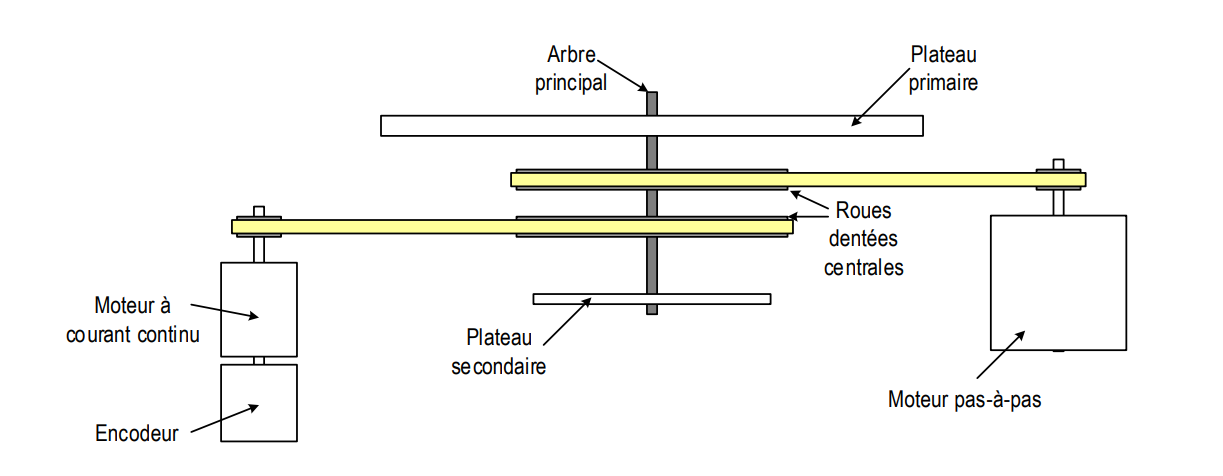
\includegraphics[width=1\linewidth]{Images/Systeme.png}
    \caption{Schéma de la maquette utilisée}
    \label{fig:systeme}
\end{figure}

\newpage
\section{Partie Théorique}
\subsection{Calculs d'inertie}
Afin de pouvoir déterminer les couples nécessaires à la réalisation des profils de vitesse imposés, il est indispensable d’évaluer l’inertie équivalente du système entraîné par le moteur pas-à-pas. Cette inertie totale rapportée au moteur, notée $J_{m,\text{tot}}$, résulte de la contribution des moteurs, du codeur, ainsi que de l’ensemble des éléments mécaniques en rotation dans la chaîne de transmission.

Les données relatives aux moteurs, au codeur incrémental et à la transmission sont extraites des fiches techniques fournies et résumées dans le Tableau~\ref{tab :donnees_moteur}. Les dimensions géométriques et les matériaux des différentes pièces mécaniques de l’axe principal sont quant à eux donnés dans le Tableau~\ref{tab :Geometrie_inertie}.
\begin{table}[h!]
\centering
\begin{tabular}{|l| c| c|}
\hline
Description & Unité & Valeur \\
\hline
Inertie moteur pas-à-pas & g·cm$^2$ & 77 \\
\hline
Inertie moteur DC & kg·m$^2$ & $6.1 \times 10^{-7}$ \\
\hline
Facteur de tension $k_u$ moteur DC & V / 1000 rpm & 7.2 \\
\hline
Inertie codeur moteur DC & g·cm$^2$ & 0.4 \\
\hline
Nombre de dents petite roue & -- & 15 \\
\hline
Nombre de dents grande roue & -- & 75 \\
\hline
Rapport de transmission $i$ & -- & 5 \\
\hline
Rendement $\eta$ & \% & 88.5 \\
\hline
\end{tabular}
\caption{Données des moteurs et de la transmission}
\label{tab :donnees_moteur}
\end{table}
\begin{table}[h!]
\centering
\begin{tabular}{|l| c| c| c| c| c|}
\hline
Élément & Matériau & $R_{ext}$ [mm] & $R_{int}$ [mm] & $H$ [mm] & $\rho$ [kg/m$^3$] \\
\hline
Plateau principal & PMMA & 95 & 3 & 5 & 1880 \\
 & Alu & 6 & 3 & 10 & 2700 \\
 & Alu & 20 & 3 & 5 & 2700 \\
 \hline
Axe vertical & Acier & 3 & -- & 55 & 7850 \\
 & Acier & 5 & -- & 60 & 7850 \\
 \hline
Roue dentée (2x) & Alu & 29.5 & 3 & 9 & 2700 \\
 & Alu & 10 & 3 & 5 & 2700 \\
 \hline
Roulements (2x) & Acier & 15 & 8 & 7 & 7850 \\
\hline
Plateau secondaire & PMMA & 20 & 3 & 2 & 1880 \\
 & Alu & 15 & 3 & 3 & 2700 \\
 & Alu & 7.5 & 3 & 8 & 2700 \\
\hline
\end{tabular}
\caption{Caractéristiques géométriques des éléments de l’axe principal}
\label{tab :Geometrie_inertie}
\end{table}
\subsubsection{Inerties des moteurs et du codeur}

Les inerties propres au moteur pas-à-pas, au moteur à courant continu utilisé comme capteur de vitesse, ainsi qu’au codeur incrémental sont extraites des fiches techniques fournies. L’inertie du moteur DC est convertie dans des unités cohérentes avec le reste des calculs. En tenant également compte de l’inertie de la petite roue dentée montée sur l’axe du moteur, les inerties des axes moteurs s’écrivent :

\begin{equation}
J_{DC} = J_{\text{mot,DC}} + J_{\text{codeur}} + J_{\text{roue}} = 6.92 \; \text{g·cm}^2
\end{equation}

\begin{equation}
J_{\text{PàP}} = J_{\text{mot,PàP}} + J_{\text{roue}} = 77.42 \; \text{g·cm}^2
\end{equation}

\subsubsection{Inerties des éléments mécaniques}

Les éléments mécaniques entraînés par l’axe principal comprennent les plateaux, l’axe vertical, les roues dentées et les roulements. Ces composants possèdent des masses non négligeables et doivent donc être pris en compte dans le calcul de l’inertie globale.

Chaque pièce est modélisée soit comme un cylindre plein, soit comme un cylindre creux selon sa géométrie. Les inerties sont calculées à l’aide des relations suivantes :

\begin{equation}
J_{\text{cylindre plein}} = \frac{1}{2} m R_{\text{ext}}^2
\end{equation}

\begin{equation}
J_{\text{cylindre creux}} = \frac{1}{2} m \left( R_{\text{ext}}^2 + R_{\text{int}}^2 \right)
\end{equation}

Les masses sont déterminées à partir des dimensions géométriques et des masses volumiques des matériaux indiquées dans le Tableau~2. La somme des inerties de l’ensemble des éléments de l’axe principal conduit à une inertie totale :

\begin{equation}
J_{\text{axe}} = 12745.7 \; \text{g·cm}^2
\end{equation}

\subsubsection{Réduction des inerties au moteur pas-à-pas}

Le système comporte plusieurs axes reliés par des transmissions à courroie. Afin de déterminer l’inertie équivalente vue par le moteur pas-à-pas, les inerties des différents axes sont ramenées à cet axe en tenant compte du rapport de transmission $i = 5$ et du rendement $\eta = 0.885$.

L’inertie totale ramenée au moteur pas-à-pas s’exprime alors comme :

\begin{equation}
J_{m,\text{tot}} =
J_{\text{PàP}}
+ \frac{J_{\text{axe}}}{\eta \, i^2}
+ \frac{J_{DC}}{\eta^2 \, i^4}
\end{equation}

En remplaçant par les valeurs numériques obtenues :

\begin{equation}
J_{m,\text{tot}} =
77.42
+ \frac{12745.7}{0.885 \cdot 25}
+ \frac{6.92}{0.885^2 \cdot 625}
\end{equation}

On obtient finalement :

\begin{equation}
\boxed{
J_{m,\text{tot}} \approx 662.3 \; \text{g·cm}^2
}
\end{equation}

Cette inertie équivalente sera utilisée dans la suite du laboratoire pour le calcul des couples moteurs nécessaires lors des phases d’accélération et de décélération.
\subsection{Profils de vitesse}
Dans cette section, les profils de vitesse utilisés lors de la partie expérimentale sont analysés et leurs caractéristiques théoriques sont déterminées. Trois profils de vitesse trapézoïdaux symétriques sont considérés. Chaque profil est défini par une phase d’accélération à accélération constante, une phase à vitesse maximale constante, puis une phase de décélération à accélération constante opposée.  

Pour tous les profils étudiés, la durée totale du mouvement ainsi que le déplacement angulaire total sont identiques. Les valeurs imposées sont les suivantes :
\begin{equation}
t_{\text{mouv}} = 0.75 \; \text{s}
\qquad
\Theta_{\text{plateau}} = 90^\circ
\end{equation}

En tenant compte du rapport de transmission entre le plateau principal et le moteur pas-à-pas, égal à $i = 5$, le déplacement angulaire total du moteur s’écrit :
\begin{equation}
\Theta_{\text{tot}} = i \cdot \Theta_{\text{plateau}}
= 5 \cdot 90^\circ
= 450^\circ
= \frac{5\pi}{2} \; \text{rad}
\end{equation}

Les profils de vitesse sont décrits à l’aide de fractions $p_1$, $p_2$ et $p_3$ correspondant respectivement aux phases d’accélération, de vitesse constante et de décélération, exprimées en fraction de la durée totale du mouvement. La répartition des profils étudiés est donnée dans le Tableau~\ref{tab:profils}.

\begin{table}[h]
\centering
\renewcommand{\arraystretch}{1.5}
\begin{tabular}{|c|c|c|c|}
\hline
 & $p_1$ & $p_2$ & $p_3$ \\
\hline
Profil 1 & $\frac{1}{3}$ & $\frac{1}{3}$ & $\frac{1}{3}$ \\
\hline
Profil 2 & $\frac{1}{4}$ & $\frac{1}{2}$ & $\frac{1}{4}$ \\
\hline
Profil 3 & $\frac{1}{8}$ & $\frac{3}{4}$ & $\frac{1}{8}$ \\
\hline
\end{tabular}
\caption{Répartition des profils de vitesse}
\label{tab:profils}
\end{table}


Ces profils étant symétriques, l’accélération maximale est égale en valeur absolue à la décélération maximale. Les durées des différentes phases s’écrivent :
\begin{equation}
t_1 = p_1 T, \qquad
t_2 = p_2 T, \qquad
t_3 = p_3 T
\end{equation}

où $T = t_{\text{mouv}}$.

Le déplacement angulaire total peut être obtenu en intégrant la vitesse sur toute la durée du mouvement. Pour un profil trapézoïdal symétrique, on obtient :
\begin{equation}
\Theta_{\text{tot}} =
\frac{1}{2}\Omega_{\max} t_1
+ \Omega_{\max} t_2
+ \frac{1}{2}\Omega_{\max} t_3
\end{equation}

ce qui peut se réécrire sous la forme :
\begin{equation}
\Theta_{\text{tot}} =
\Omega_{\max}
\left(
-\frac{1}{2}t_3 + t_3 + t_2 + \frac{1}{2}t_1
\right)
\end{equation}

La vitesse maximale du moteur est alors donnée par :
\begin{equation}
\Omega_{\max} =
\frac{\Theta_{\text{tot}}}
{
-\frac{1}{2}t_3 + t_3 + t_2 + \frac{1}{2}t_1
}
\end{equation}

L’accélération maximale est obtenue à partir de la relation de mouvement circulaire uniformément accéléré :
\begin{equation}
\alpha_{\max} = \frac{\Omega_{\max}}{t_1}
\end{equation}

La vitesse angulaire moyenne du moteur, identique pour les trois profils puisque le déplacement total et la durée sont constants, est définie par :
\begin{equation}
\Omega_{\text{moy}} = \frac{\Theta_{\text{tot}}}{T}
\end{equation}

En remplaçant par les valeurs numériques, on obtient :
\begin{equation}
\Omega_{\text{moy}} =
\frac{5\pi/2}{0.75}
= 10.47 \; \text{rad·s}^{-1}
\end{equation}

Les valeurs de vitesse maximale, d’accélération maximale et de vitesse moyenne obtenues pour chacun des profils sont regroupées dans le Tableau~\ref{tab:valeurs_profils}.

\begin{table}[h]
\centering
\begin{tabular}{|c|c|c|c|}
\hline
Profil & $\Omega_{\max}$ [rad/s] & $\alpha_{\max}$ [rad/s$^2$] & $\Omega_{\text{moy}}$ [rad/s] \\
\hline
Profil 1 (1/3--1/3--1/3) & 15.71 & 62.8 & 10.47 \\
Profil 2 (1/4--1/2--1/4) & 13.97 & 74.5 & 10.47 \\
Profil 3 (1/8--3/4--1/8) & 11.97 & 127.7 & 10.47 \\
\hline
\end{tabular}
\caption{Valeurs théoriques des profils de vitesse}
\label{tab:valeurs_profils}
\end{table}

Ces résultats montrent que, bien que la vitesse moyenne reste constante pour tous les profils, les accélérations maximales augmentent lorsque la durée des phases d’accélération et de décélération diminue. Ces accélérations auront une influence directe sur le couple maximal requis au niveau du moteur pas-à-pas, qui sera analysé dans la section suivante.



\subsection{ Calcul des valeurs de programmation}
Afin de piloter correctement le moteur pas-à-pas pour réaliser les profils de mouvement calculés précédemment, il est nécessaire de déterminer les paramètres à programmer dans l’électronique de commande. Ces paramètres incluent notamment : \texttt{velocity}, \texttt{amax}, \texttt{Position} (ou \texttt{Temps}), \texttt{pulse\_div}, \texttt{ramp\_div} et \texttt{Usrs}.

\subsubsection{Fréquence des micro-pas}

La première étape consiste à calculer la fréquence des micro-pas \(f_{\text{usf}}\) [Hz], qui dépend de la résolution des micro-pas définie par \texttt{Usrs}. Pour notre cas, la résolution choisie est :
\[
\text{Usrs} = 6 \quad \Rightarrow \quad 64 \text{ micro-pas par pas entier}.
\]

La fréquence des micro-pas est calculée à partir de la fréquence de l’horloge interne \(f_{\text{CLK}}\), du nombre de pas par tour \(N\) et de la vitesse de pas entière (\texttt{velocitymax}) selon la relation suivante :
\begin{equation}
f_{\text{usf}} = \frac{N \cdot \text{velocitymax} \cdot 2}{\text{Usrs}}
\end{equation}

\subsubsection{Pré-diviseur de vitesse \texttt{pulse\_div}}

Le paramètre \texttt{pulse\_div} permet d’adapter la vitesse maximale du moteur à la fréquence des micro-pas. Il est calculé par :
\begin{equation}
\text{pulse\_div} = \log_2 \left( \frac{f_{\text{CLK}} \cdot \text{velocitymax}}{f_{\text{usf}} \cdot 2048 \cdot 32} \right)
\end{equation}
Cette valeur est arrondie à l’entier inférieur. Elle est ensuite utilisée pour recalculer la vitesse maximale réelle à programmer :
\begin{equation}
\text{velocity} = \frac{f_{\text{usf}} \cdot 2^{\text{pulse\_div}}}{2048 \cdot 32} \cdot \frac{1}{f_{\text{CLK}}}
\end{equation}
La vitesse est arrondie à l’entier supérieur tant que sa valeur reste inférieure à \texttt{velocitymax}.

\subsubsection{Accélération et pré-diviseur de rampe \texttt{ramp\_div}}

L’accélération angulaire maximale en micro-pas est calculée à partir de l’accélération maximale du moteur (\(\alpha_{\max}\)) et de la résolution des micro-pas :
\begin{equation}
a = \text{résolution} \cdot \frac{\alpha_{\max}}{2\pi} \; [\text{Hz/s}]
\end{equation}

Le paramètre \texttt{ramp\_div} est ensuite calculé comme :
\begin{equation}
\text{ramp\_div} = \log_2 \left( \frac{f_{\text{CLK}}^2 \cdot \text{amax}}{a} \right) - \text{pulse\_div} - 29
\end{equation}

La valeur arrondie à l’entier inférieur permet ensuite de recalculer la valeur effective de l’accélération à programmer :
\begin{equation}
a = \frac{f_{\text{CLK}}^2 \cdot \text{amax}}{2^{\text{pulse\_div} + \text{ramp\_div} + 29}}
\end{equation}
Cette valeur est arrondie à l’entier supérieur tant qu’elle reste inférieure à \texttt{amax}.

\subsubsection{Consigne de position et temps}

Si le moteur est contrôlé en position angulaire, la consigne \(\vartheta_c\) [pas] est calculée par :
\begin{equation}
\vartheta_c = \frac{N \cdot 2}{\text{Usrs}} \cdot \frac{\vartheta}{360}
\end{equation}
où \(\vartheta\) est l’angle cible en degrés.  

Si le moteur est contrôlé en temps, le paramètre \texttt{Temps} correspond à la durée totale du mouvement exprimée en tranches de 10 ms :
\begin{equation}
\text{Temps} = T[\text{s}] \cdot 100
\end{equation}

\subsubsection{Variables à programmer}

Le Tableau~\ref{tab:variables_prog} résume les principales variables à entrer dans le programme de l’électronique pour obtenir le profil de mouvement souhaité.

\begin{table}[h]
\centering
\renewcommand{\arraystretch}{1.3}
\begin{tabular}{|c|c|c|c|c|c|}
\hline
Nom & Description & N° param. & Gamme & Valeur par défaut & Unité \\
\hline
fCLK & Fréquence de l’horloge & --- & --- & 16 & MHz \\
velocity & Vitesse maximale & 4 & 0 … 2047 & 1000 & [-] \\
amax & Accélération maximale & 5 & 0 … 2047 & 1000 & [-] \\
pulse\_div & Pré-diviseur vitesse & --- & 0 … 13 & 3 & [-] \\
ramp\_div & Pré-diviseur rampe & 153 & 0 … 13 & 7 & [-] \\
Usrs & Résolution micro-pas & 140 & 0 … 6 & 6 & [-] \\
N & Nombre de pas par tour & --- & --- & 200 & pas/tr \\
\hline
\end{tabular}
\caption{Variables de programmation pour l’électronique du moteur}
\label{tab:variables_prog}
\end{table}

Le Tableau~\ref{tab:Usrs} donne la correspondance entre la valeur de \texttt{Usrs} et le nombre réel de micro-pas par pas entier.

\begin{table}[h]
\centering
\renewcommand{\arraystretch}{1.3}
\begin{tabular}{|c|c|}
\hline
Usrs & Nombre de micro-pas \\
\hline
0 & 1 (pas entier) \\
1 & 2 (demi-pas, non recommandé) \\
2 & 4 \\
3 & 8 \\
4 & 16 \\
5 & 32 \\
6 & 64 \\
7 & 128 \\
8 & 256 \\
\hline
\end{tabular}
\caption{Nombre de micro-pas en fonction de la valeur de Usrs}
\label{tab:Usrs}
\end{table}

Ces calculs permettent de programmer correctement la vitesse, l’accélération et la position (ou le temps) afin que le moteur exécute les profils de mouvement souhaités de manière précise et fiable. Les ajustements éventuels de \texttt{pulse\_div} et \texttt{ramp\_div} peuvent être faits par incréments unitaires pour optimiser le comportement réel du moteur.


\newpage
\section{Méthode de mesure}
\subsection{Liste de matériel}
\begin{itemize}
    \item Maquette N°1 : moteur pas-à-pas QMOT
    \item Oscilloscope Tektronix DPO2014B, n°C011149.
     \item Câbles RS-232 pour connexion au module
    \item Alimentation 24V pour le moteur
    \item Logiciel TMCL pour programmation du module
    \item Fichiers TMCL de base : \texttt{TMCL.exe} et \texttt{MOV\_vide.tmc}
\end{itemize}
\subsection{Procédure de mesure}
\begin{enumerate}
    \item \textbf{Identification du moteur} : relever le numéro de maquette et identifier la référence du moteur pas-à-pas.
    
    \item \textbf{Programmation du module TMCL} :  
    Télécharger et ouvrir les fichiers TMCL, identifier le port COM et établir la connexion. Paramétrer le courant selon le moteur, compiler (\texttt{Assemble}) et charger (\texttt{Download}) le programme. Utiliser \texttt{Run} et \texttt{Stop} pour contrôler le mouvement.

    \item \textbf{Vérification des calculs} :  
    Vérifier les valeurs calculées de \texttt{pulse\_div}, \texttt{velocity}, \texttt{ramp\_div}, \texttt{amax} et \(\vartheta_C\) via Setup → Parameter Calculation.

    \item \textbf{Essais des profils} :  
    Compléter \texttt{MOV\_vide.tmc} pour exécuter les profils, visualiser la vitesse sur l’oscilloscope et comparer avec les valeurs théoriques.

    \item \textbf{Réduction du temps de mouvement} :  
    Recalculer les paramètres pour des temps de 0.12 s à 0.08 s (pas de 0.01 s) et tracer les courbes pull-out pour identifier le temps minimal où le moteur suit la consigne.

    \item \textbf{Micro-pas vs pas entiers (bonus)} :  
    Pour le profil 1/6--2/3--1/6, recalculer les paramètres avec \texttt{Usrs = 0} pour 0.75 s et comparer le signal de vitesse avec celui en micro-pas.
\end{enumerate}

Cette méthode permet d’évaluer le comportement dynamique du moteur, de vérifier les calculs théoriques et de déterminer ses limites de performance.
\newpage
\section{Résultats expérimentaux}
\subsection{Visualisation des profils de mouvement}
\subsubsection{Profil de mouvement $\frac{1}{2} \frac{1}{2} \frac{1}{2}$}
\begin{figure}[H]
    \centering
    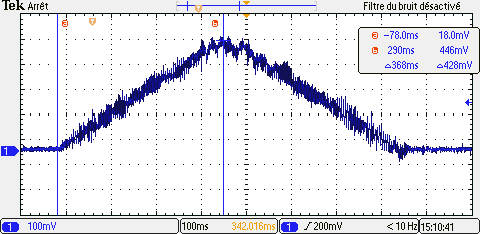
\includegraphics[width=1\linewidth]{Images/PM_triangle_0.75s.PNG}
    \caption{Profil de mouvement $\frac{1}{2} \frac{1}{2} \frac{1}{2}$}
    \label{fig:triangle}
\end{figure}
\subsubsection{Profil de mouvement $\frac{1}{3} \frac{1}{3} \frac{1}{3}$}
\begin{figure}[H]
    \centering
    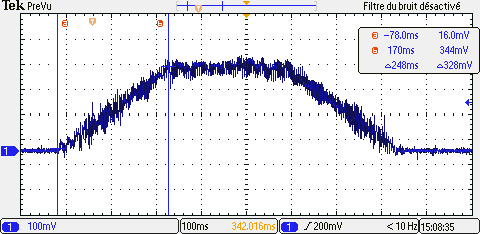
\includegraphics[width=1\linewidth]{Images/PM131313_075s.PNG}
    \caption{Profil de mouvement $\frac{1}{3} \frac{1}{3} \frac{1}{3}$ }
    \label{fig:131313}
\end{figure}
\subsubsection{Profil de mouvement $\frac{1}{6} \frac{2}{3} \frac{1}{6}$}
\begin{figure}[H]
    \centering
    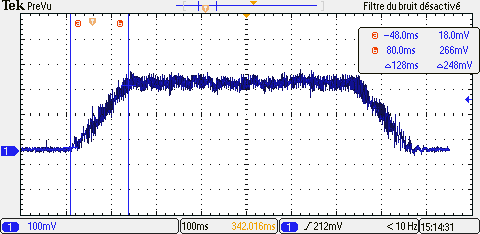
\includegraphics[width=1\linewidth]{Images/PM_162316_075s.PNG}
    \caption{Profil de mouvement $\frac{1}{6} \frac{2}{3} \frac{1}{6}$ }
    \label{fig:162316}
\end{figure}
\subsection{Réduction du temps de mouvement}
\subsection{Bonus : Comparaison de fonctionnement entre micro-pas et pas entiers}
\begin{figure}[H]
    \centering
    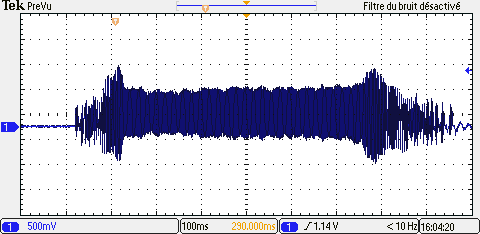
\includegraphics[width=1\linewidth]{Images/bonus_1.PNG}
    \caption{Fonctionnement en pas entiers}
    \label{fig:profil_bonus}
\end{figure}
\begin{figure}
    \centering
    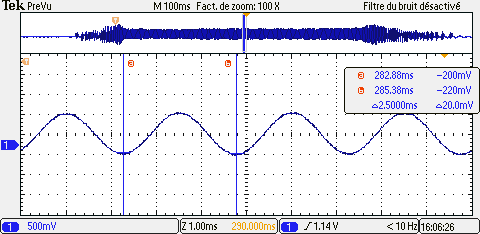
\includegraphics[width=1\linewidth]{Images/bonus_2.PNG}
    \caption{Fréquence d'oscillation en pas entiers}
    \label{fig:freq_bonus}
\end{figure}
\newpage
\input{chapitres/Analyse des résultats}
\newpage
\input{chapitres/apport}
\newpage

\section{Conclusion}

Ce projet a permis de mener une démarche complète de conception d’un robot SCARA parallèle à mécanisme plan à cinq barres.
\newline
À partir du cahier des charges initial, une solution mécanique complète a été développée en tenant compte des contraintes fonctionnelles, mécaniques, de fabrication et de montage.
\newline
L’analyse du besoin a permis de définir les fonctions principales du système ainsi que les contraintes à respecter, notamment la zone de travail, l’encombrement, la masse, la rigidité et l’intégration des actionneurs. 
Ces éléments ont guidé les choix de conception tout au long du projet et ont permis de converger vers une architecture cohérente avec les objectifs fixés.
\newline
Le choix d’une architecture parallèle avec moteurs placés sur la partie fixe s’est révélé pertinent pour limiter les masses en mouvement et améliorer le comportement dynamique du robot. La transmission par courroies et poulies permet quant à elle de déporter l’entraînement tout en conservant une solution simple et adaptée à l’encombrement disponible.

Le dimensionnement des principaux composants a permis de valider la faisabilité mécanique du système. Les bras, les arbres, les roulements, les poulies, les courroies et les actionneurs ont été sélectionnés en fonction des efforts transmis, des contraintes d’intégration et des exigences de fonctionnement. Cette étape a également permis de vérifier que les composants choisis sont compatibles avec une réalisation à partir d’éléments standards et de pièces fabriquées.

Une attention particulière a été portée à l’assemblage du robot. La conception des sous-ensembles a été pensée en tenant compte de l’ordre de montage, de l’accessibilité des vis, du positionnement des roulements, des circlips, des accouplements et des courroies. Cette réflexion a permis de rendre le système plus réaliste à fabriquer, à assembler et à maintenir.
\newline
\newline
Le projet a également intégré une réflexion sur l’esthétique globale du robot. Comme le système est destiné à servir de support de démonstration, il était important de proposer une solution fonctionnelle, mais aussi propre, lisible et visuellement cohérente. L’intégration des moteurs, des transmissions, des bras et de la structure a donc été pensée afin d’obtenir un ensemble soigné.

Au-delà de la conception mécanique elle-même, ce projet a permis de développer une vision plus globale du travail d’ingénierie. Il a nécessité de faire des choix techniques, de les justifier, de dimensionner les composants, mais aussi de penser à la fabrication, au montage, à l’utilisation et à l’apparence finale du système. Il a ainsi regroupé de nombreux aspects complémentaires d’un projet réel de conception.
\newline
\newline
En conclusion, le travail réalisé a permis d’aboutir à une conception complète et cohérente du robot. Les solutions retenues répondent aux principales exigences du cahier des charges et constituent une base solide pour la fabrication, l’assemblage et les essais du système.



\newpage
\begin{thebibliography}{9}
\label{bib}

\bibitem{BossoneyLabo}
Prof. L. Bossoney,  
\textit{Systèmes électromécaniques, Labo : Entraînement à moteur pas-à-pas},  
HEIG-VD, Yverdon-les-Bains.

\bibitem{BossoneyCours}
Prof. L. Bossoney,  
\textit{Cours de systèmes électromécaniques},  
HEIG-VD, Yverdon-les-Bains, 2021.

\end{thebibliography}

\vspace{2cm}  % espace avant la signature
\noindent
Fait à : \textbf{Yverdon-les-Bains le \today} 

\vspace{2cm}  % espace avant les signatures
\noindent
\begin{tabular}{l l}

\includegraphics[height=5cm]{logos/Salma_sign.png} &  \hspace{3.75cm} 
\includegraphics[height=2cm]{logos/SignatureJG.jpg} \\
Salma Elmnouar & \hspace{5cm} Julien Golaz
\end{tabular}

\newpage
\input{chapitres/Annexes}
\end{document}